\documentclass[a4paper,11pt]{article}
\usepackage[T1]{fontenc}
\usepackage[utf8]{inputenc}
\usepackage{lmodern}

\usepackage{makeidx}
    % Needed to build the index.

\usepackage{amsmath}
    % Brings the align environment for lining up equations on the =.

\usepackage{amssymb}
    % For the number set symbols.

\usepackage{cancel}
    % For striking out bits of equations that simplify.

\usepackage{graphicx}
    % Can't have pictures/photos/figures from files without that.
    % Note that vanilla latex will only accept eps.
    
\usepackage{subfigure}
    % Lets me have labels such as a) b) c) inside a figure environment.

\usepackage[font=footnotesize, labelfont=bf]{caption}
    % So that I can add long captions under figures.
    % It provides me with \caption* that does not appear in the list of
    % figures but formats the text like \caption does.  It also lets me
    % use line breaks in the caption, and even bullet/enumerated lists.

\usepackage{color}
    % For rendering text is eps_tex files produced by InkScape, even
    % if the text is black.

\usepackage{booktabs}
    % For professional-looking tables.
    % Brings the \toprule, \midrule and \bottomrule.
    % Remember not to use vertical rules in tables: they look cheap.

\usepackage[version=3]{mhchem}
    % For chemical formulas.
    % Brings \ce.ormulas.

\usepackage{stmaryrd}
    % For the llbracket and rrbracket to denote integer intervals.

\usepackage{varioref}
    % For fancier references that also tell the page number.
    
\usepackage{todonotes}
    % Big post-its, handy while writing.
    
\usepackage[]{biblatex}
    % Fantastic bibliography manager that I'll use just for its
    % \citetitle command.

%\usepackage[mediumspace,mediumqspace,squaren]{SIunits}
\usepackage{siunitx}
    % Otherwise I can't write the mu symbol for micrometers.
    % It also brings me the \degree symbol, woo!
    % No decibel though, I need to make this one myself.
\newcommand{\decibel}{dB}
\newcommand{\equaldef}{\stackrel{\text{\tiny def}}{=}}
\newcommand{\transp}{^T}
\newcommand{\norm}[1]{\left\| #1 \right\|}
\newcommand{\abs}[1]{\left| #1 \right|}

\graphicspath{{./figures/}}
\addbibresource{bibliography.bib}

\title{Understanding standing waves by network modeling
\\
\large{HIFI untangled, and prospects for future instrumentation}}
\author{Bertrand Delforge$^{1, 2}$
       \and
       John Pearson$^3$
       \and
       Marc Verheijen$^2$
       \and
       Peter Roelfsema$^1$
       \and
       Willem Jellema$^1$
       \and
       \\ \footnotesize $^1$ SRON, Netherlands Institute for Space Research
       \\ \footnotesize $^2$ Kapteyn Astronomical Institute
       \\ \footnotesize $^3$ JPL, Jet Propulsion Laboratory
}

\begin{document}

\maketitle
%\tableofcontents

\begin{abstract}
As is the case for many instruments like HIFI, the Heterodyne Instrument for the Far Infrared on the Herschel space observatory, standing waves affect the nominal coupling of the mixer to the local oscillator, calibration black bodies and even the sky.  This results in obvious distortions of the spectral baselines and strongly influences less obvious measures such as the sideband ratio.  Current uncertainties on HIFI's sideband ratio are about 2-10 percent, depending on the frequency, and are mainly a consequence of an insufficient understanding of the HIFI standing wave phenomenon.

We are developing a systematic and generic methodology for modeling standing waves in coherent optical and quasi-optical systems, using scattering matrices of Jones matrices.  This approach allows for a correct processing of the phase and polarization information of multi-port networks, and serves as a foundation for a framework that combines an arbitrarily large number of networks and predicts their interactions.

Our numerical simulations successfully reproduce, and qualitatively explain, many artifacts observed in actual HIFI data while we are currently improving our technique to produce quantitative predictions.  With HIFI as a hands-on show case for our successful standing wave modeling technique, we are confident that our generic approach for understanding and predicting standing waves can play a significant role in improving the design of future instruments.
\end{abstract}





%=============================================================================

\section{Introduction}
The HIFI instrument on the Herschel Space Observatory \cite{AA_518_L1} operates at frequencies between \SI{480}{\giga\hertz} and \SI{1910}{\giga\hertz}
and produces spectra with a resolution ranging from \SI{1}{\mega\hertz} to \SI{125}{\kilo\hertz} \cite{AA_518_L6}.
This high frequency resolution enables the study the chemistry of a wide range of phenomena, from planetary atmosphere to star forming regions.

At such a high resolution, the thermal noise of the astronomical source and that of the calibration black bodies and local oscillator (LO) qualify as ``narrow band Gaussian noise signal'' \cite{siegman1986lasers} and have a coherence time $\tau$ equal to the inverse of their bandwidth~$\tau=1/\Delta f$.
A bandwith of~\SI{1}{\mega\hertz} results in a coherence time of \SI{1}{\micro\second} or, when multiplied by the speed of light, a coherence length of \SI{300}{\meter} which is a hundred times the longest distance inside HIFI.
Therefore, in HIFI, both the LO signal and the signals from the sources are coherent.

Coherence allows for interferences.
Interferences inside electromagnetic cavities give birth to standing waves which trap energy inside these cavity.
The mixer cannot detect the energy that is trapped; 
therefore the coupling of the incoming signals to the mixer is modulated by these standing waves.

\begin{figure}[hbt]
    \centering
    % CO 9-8 line of NCG7538-IRS1 observed on 21-02-2010.
    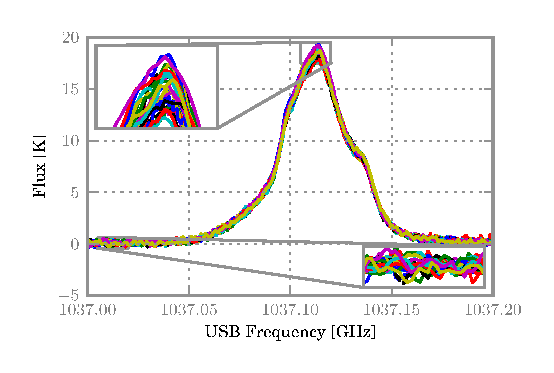
\includegraphics{obsid_5000352C}
    \caption{\label{fig:scatter_real_data}
    The same extragalactic emission feature observed by HIFI at 25 different LO frequencies in its band 4a.
    If the calibration were perfect, all these line profiles would overlap within the noise.
    However, after subtracting the baseline, we observe a scatter on the line peak intensity that has a standard deviation three times greater than the expected noise (which is represented by the error bars).
    This scatter is due to standing waves that are ignored by the calibration: each LO frequency requires a specific tuning of the diplexer, which changes the optical path and therefore the periods of the standing waves, modulating the coupling of the mixer to the sky, LO and calibration loads.
    Our objective is to model the complex relationship between parameters such as the LO frequency and the coupling modulation due to standing waves.
    }
\end{figure}

Figure~\ref{fig:scatter_real_data} illustrates this phenomenon.
HIFI observed a single emission feature from a galactic source.
It did so 25 times for 25 local oscillator frequencies.
This is an engineering observation designed to show subtle standing waves effects.
Even though each of these 25 spectra looks individually clean from standing wave modulations (no apparent periodic distortion of the spectrum), their comparison shows that standing waves cause an uncertainty on the peak amplitude of the line.
In that specific case, the uncertainty due to standing waves is three times greater than that due to the noise.
In other terms, almost half of the observing time is invested in reducing the noise below the standing-wave uncertainty, which cannot be reduced by longer integration times.
When an observation is taken at one LO frequency only, the astronomer has little to no way of knowing how much standing waves distort the line.

This motivates the present work.
Our goal is to model the instrument to a level which allows to accurately predict the effect of the standing waves, and include a correction of their effect in the calibration scheme of HIFI.





%=============================================================================

\section{Modeling standing waves}



%-----------------------------------------------------------------------------

\subsection{Principle}
Our method is inspired from laser and circuit theory: we deal with discrete inputs and outputs rather than, for example, a continuous description of the fields in space.
A system like the Focal Plane Unit of HIFI comprises a few dozens of optical elements, also called ``networks'': wire grid polarizers, roof-top mirrors, horns, attenuators, free space, all having one or more input and output.
All these networks interact together two by two since there exists at least one optical path between each pair or networks.
The number of interactions in the system increases with the square of the number of networks.
One way to solve a system's reaction to a set of input would be to propagate the inputs from network to network, back and forth, until the fields appear to converge to a steady state.
Instead, we propose a method to reduce the number of networks without losing any information, in a way that can be compared to calculating the equivalent impedance of an electric circuit.
Our model computes the scattering matrix of the network equivalent to the whole system.
Then, knowing how the system reacts to an input is merely a matter of multiplying its scattering matrix with a vector of inputs to get a vector of outputs\footnote{The LO output and the sky/blackbody output must be calculated separately and added in the end even though both use the same scattering matrix: each is coherent, but they are not phase-locked to each other and therefore do not interfere together}.

Scattering matrices \cite{siegman1986lasers} model the transfer of energy or field from one side (port) of a network to another (figure~\ref{fig:ports}).
\begin{figure}[hbtp]
    \centering
    \input{figures/scattering_matrix_notations.eps_tex}
    \caption{\label{fig:ports}A 4-ports network showing 4 inputs $a_i$ and four outputs $b_i$.  For example, this network could be a wire grid polarizer or a semi-transparent mirror, both acting as beam splitters.}
\end{figure}
Equation~\ref{eq:scattering_matrix} presents the scattering matrix $S$ that models the relation between a vector of inputs $a$ and a vector of outputs $b$ for a $n$-ports network.
The diagonal contains the reflections terms and the rest contains the transmissions.
\begin{align}
    b &= S a
    &
    \begin{pmatrix}
        b_1\\
        b_2\\
        \vdots\\
        b_n
    \end{pmatrix}
    &=
    \begin{pmatrix}
        S_{1, 1} & S_{1, 2} & \cdots & S_{1, n} \\
        S_{2, 1} & S_{2, 2} & \cdots & S_{2, n} \\
        \vdots   & \vdots   & \ddots & \vdots   \\
        S_{n, 1} & S_{n, 2} & \cdots & S_{n, n}
    \end{pmatrix}
    \begin{pmatrix}
        a_1\\
        a_2\\
        \vdots\\
        a_n
    \end{pmatrix}
    \label{eq:scattering_matrix}
\end{align}
The standard way to include the polarization into a scattering matrix is to double (local reference frame: horizontal and vertical directions) or triple (global reference frame: $x$, $y$ and $z$ directions) its number of ports.
For our model, we chose a different approach that allows us consider a polarized field as a single entity instead of two or three, and keep the number of ports to a minimum.
For this, we decided that the elements of the scattering matrix be Jones matrices and not scalars.

Jones matrices model the transfer of amplitude and phase from one polarization to another \cite{hecht2002optics}.
Putting 3D Jones matrices inside scattering matrices is a natural way of doing both the port-to-port and the polarization energy transfer at the same time.
In equation~\eqref{eq:jones_matrix_short}, the polarized input field $e_i$ is related to the polarized output field~$e_o$ by the Jones matrix $J$.
As shown in equations~\eqref{eq:jones_matrix}, Jones matrices traditionally work in 2D~\eqref{eq:jones_matrix_2d} but it is trivial to extend them to work in 3D~\eqref{eq:jones_matrix_3d}.
Each $S_{i, j}$ is a 3D Jones matrix; each $a_j$ and each $b_i$ are 3D Jones vectors.
\begin{subequations}    
    \begin{align}
        % Small form.
        e_o &= J e_i
        \label{eq:jones_matrix_short}
        \\
        % Jones matrix in 2D.
        \begin{pmatrix}
            e_{o, h}\\
            e_{o, v}
        \end{pmatrix}
        &=
        \begin{pmatrix}
            J_{h, h}   &   J_{h, v} \\
            J_{v, h}   &   J_{v, v}
        \end{pmatrix}
        \begin{pmatrix}
            e_{i, h}\\
            e_{i, v}
        \end{pmatrix}
        \label{eq:jones_matrix_2d}
        \\
        % Jones matrix in 3D.
        \begin{pmatrix}
            e_{o, x}\\
            e_{o, y}\\
            e_{o, z}
        \end{pmatrix}
        &=
        \begin{pmatrix}
            J_{x, x}   &   J_{x, y}   &   J_{x, z} \\
            J_{y, x}   &   J_{y, y}   &   J_{y, z} \\
            J_{z, x}   &   J_{z, y}   &   J_{z, z}
        \end{pmatrix}
        \begin{pmatrix}
            e_{i, x}\\
            e_{i, y}\\
            e_{i, z}
        \end{pmatrix}
        \label{eq:jones_matrix_3d}
    \end{align}
    \label{eq:jones_matrix}
\end{subequations}
Extending Jones matrices to 3D makes it easier to work in a common reference frame in which the networks can have arbitrary orientations.
It also relieves the constraint of TEM modes and enables hybrid modes, allowing to model birefringent networks in which the electric field may have a component along the direction of propagation.
Jones matrices cannot handle non-polarized light but this is not a problem for us as wire grid polarizers ensure that everything in our system is linearly or elliptically polarized.

As shown of figure~\ref{fig:between_networks}, two networks P and Q connected by one port (port $\alpha$ for P and port $\beta$ for Q) can be seen as a single equivalent  network S.
The scattering matrix of that equivalent network takes into account the infinite reflections between the two original networks.

If we have a method to compute an equivalent network, then we can apply it recursively to an entire system to get the network equivalent to the whole system.
This is illustrated by figure~\ref{fig:cascading_example}
\begin{figure}[hbtp]
    \centering
    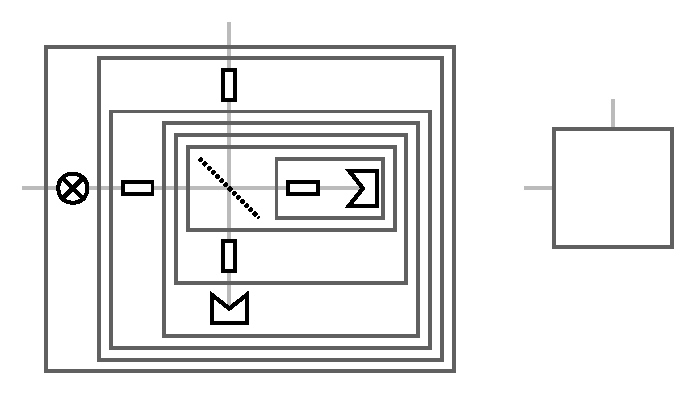
\includegraphics{cascading_example}
    \caption{\label{fig:cascading_example}
    We recursively combine networks two by two until there is only one network left.
    This example presents a HIFI diplexer unit; it contains two rooftop mirrors (pentagons) and a wire grid polarizer (dotted line) separated by free space (rectangles), its purpose is to align the polarization of the LO and the sky signals in order to couple both to the mixer (crossed circle).
    }
\end{figure}

Our method is recursive but not iterative: it passes over each network only once.
Once the scattering matrix of the whole system is calculated, we have direct access to the steady state of that system.



%-----------------------------------------------------------------------------

\subsection{Simplifications}

HIFI operates in the sub-millimeter regime where the wavelength is not much shorter than the dimensions of the networks.
We could use quasi optics to properly account for the diffraction of the beams \cite{goldsmith1998quasioptical}.
Instead, we have decided to focus on the first order effects and ignore the diffraction.
Our model assumes plane, and therefore single-mode, waves.
The plane-wave hypothesis is acceptable at a first order because the networks are placed at the waist of the beams where the wave front is plane.
Furthermore, the discrepancies due to these simplifications can be abstracted by parameters in our model.
For example, if a higher mode does not couple to a mixer, then its power is --for all practical purpose-- lost, and therefore a term of loss can model it.

Our model can be extended to higher order modes.
This can be done by adding components to the Jones vectors/matrices, or by adding an additional layer of matrices between the scattering matrix and the Jones matrix, which would take care of the transfer of energy between modes.



%-----------------------------------------------------------------------------

\subsection{Elements of modeling}
\paragraph{Chaining networks.}
\begin{figure}[hbtp]
    \centering
    \input{figures/combining_networks.eps_tex}
    \caption{\label{fig:between_networks}
        Two networks P and Q connected by one port have an equivalent network S.
        Notations used to describe two networks P and Q connected by one port:
        P~has $n_P$~ports and Q has $n_Q$~ports, here $n_P=4$ and $n_Q=3$;
        the equivalent network S has $n_S = n_P + n_Q - 2$ ports, here $n_S=5$.
        We use a common indexing scheme for the scattering matrices of P, Q and S:
        ports 1 to $n_P$ are ports of P (here 1 to 4),
        ports $n_P+1$ to $n_P+n_Q$ are ports of Q (here 5 to 7),
        ports 1 to $n_P+n_Q$ except $\alpha$ and $\beta$ are ports of S (here 1 to 7 except 3 and 5).
        The port~$\alpha$ of~P is connected to the port~$\beta$ of~Q, here $\alpha=3$ and $\beta=5$.
        Because of the connection, the output of port $\alpha$, $b_\alpha$, is equal to the input of port $\beta$ noted $a_\beta$; we name it $c$.  Likewise, we name $d$ the output of $\beta$ which is equal to the input of $\alpha$.
        The scattering matrices of P, Q and S are noted $P$, $Q$ and $S$.
        }
\end{figure}
Figure~\ref{fig:between_networks} introduces notations useful for describing the electric field between two connected networks.
In order to simplify the reasoning and shorten the equations, we use an indexing system that is common to $P$, $Q$ and $S$.  This means that the way we index our matrices is unconventional: the matrix $Q$ is indexed by port numbers ranging from $n_P+1$ to $n_P + n_Q$, therefore $Q_{1, j}$ does not exist since the port 1 does not belong to Q.  In order to write a software implementation of these equations, one level of indirection is required to transform the port numbers into conventional matrix indices.
Finally, the elements of the matrices $P$, $Q$ and $S$ are themselves matrices: they are Jones matrices.

Equation~\eqref{eq:between_networks} describes the electric field between P and Q once the steady state is established.
\begin{equation}
    \left\lbrace
    \begin{aligned}
        c
        &=
        P_{\alpha, \alpha} d + \sum_{j = 1 \atop j \neq \alpha}^{n_P}
        \left(
            P_{\alpha, j}a_j
        \right)
        \\
        d
        &=
        Q_{\beta, \beta} c + \sum_{j = n_P+1 \atop j \neq \beta}^{n_P + n_Q}
        \left(
            Q_{\beta, j}a_j
        \right)
    \end{aligned}
    \right.
    \label{eq:between_networks}
\end{equation}
In equation~\eqref{eq:between_networks}, $c$~and~$d$ depend on each other.
Equation~\eqref{eq:d} presents the solution of this system for~$d$.
\begin{equation}
    d =
    (I - Q_{\beta, \beta} P_{\alpha, \alpha})^{-1}
    \left[
        Q_{\beta, \beta}
        \sum_{j = 1 \atop j \neq \alpha}^{n_P}
        \left(
            P_{\alpha, j}
            a_j
        \right)
        +
        \sum_{j = n_P \atop j \neq \beta}^{n_P + n_Q}
        \left(
            Q_{\beta, j}
            a_j
        \right)
    \right]
    \label{eq:d}
\end{equation}
In equation~\eqref{eq:d}, $I$ represents the identity matrix that matches the size of $Q_{\beta, \beta}P_{\alpha, \alpha}$ (that is, 3--by--3 as these are 3D Jones matrices).
We are certain that $I - Q_{\beta, \beta} P_{\alpha, \alpha}$ has an inverse because the system has losses:
if it did not have an inverse then the system could store an infinite amount of energy and therefore never reach a steady state, this system would not be physical.
Since~$d$ is an input for~P, we can express the outputs of P in terms of~$d$.
\begin{gather}
\begin{aligned}
    \forall i, i
    &\in
    \left\llbracket 1 ; n_P \right\rrbracket, i \neq \alpha
    &
    b_i
    &=
    P_{i, \alpha} d
    + \sum_{j = 1 \atop j \neq \alpha}^{n_P}
    \left(
        P_{i, j}a_j
    \right)
\end{aligned}
\notag
\\
\begin{aligned}
    b_i
    &=
        \sum_{j = 1 \atop j \neq \alpha}^{n_P}
        \left[
            \left(
                P_{i, \alpha}
                (I - Q_{\beta, \beta} P_{\alpha, \alpha})^{-1}
                Q_{\beta, \beta}
                P_{\alpha, j}
                +
                P_{i, j}
            \right)
            a_j
        \right]
    \\
    &+
        \sum_{j = n_P+1 \atop j \neq \beta}^{n_P + n_Q}
        \left[
            \left(
                P_{i, \alpha}
                (I - Q_{\beta, \beta} P_{\alpha, \alpha})^{-1}
                Q_{\beta, j}
            \right)
            a_j
        \right]
\end{aligned}
\label{eq:P_side_of_S}
\end{gather}
Equation~\ref{eq:P_side_of_S} gives us what we are looking for: the outputs~$b_i$ as functions of the inputs~$a_j$.
It is however limited to what we can call the ``P-side'' of the equivalent network S: the output ports~$b_1$ to~$b_{n_P}$.
We repeat this reasoning with~$c$ and~$Q$ to get~$b_i$ for the ``Q-side'' of the equivalent network S: outputs~$b_{n_P}$ to~$b_{n_P+n_Q}$.

We have expressed the elements of~$b$ as a linear combinations of the elements of~$a$,
therefore we have all the coefficients~$S_{i, j}$ of the matrix of our equivalent network.
This matrix is divided into four sections depending on the port numbers:
$i \in \llbracket 1 ; n_Q \rrbracket$ and
$i \in \llbracket n_P + 1 ; n_P + n_Q \rrbracket$,
and the same for~$j$ as shown in table \ref{table:equivalent_network}.
\begin{table}[htbp]
    \centering
    \begin{tabular}{r|c c}
        \toprule
            $S_{i, j}$
            &
            $j \in \llbracket 1 ; n_P \rrbracket$
            &
            $j \in \llbracket n_P + 1 ; n_P + n_Q \rrbracket$ \\
        \midrule
            $i \in \llbracket 1 ; n_P \rrbracket$
            &
            $
                P_{i, \alpha}
                R_P
                Q_{\beta, \beta}
                P_{\alpha, j}
                +
                P_{i, j}
            $
            &
            $
                P_{i, \alpha}
                R_P
                Q_{\beta, j}
            $
            \\
            $i \in \llbracket n_P + 1 ; n_P + n_Q \rrbracket$
            &
            $
                Q_{i, \beta}
                R_Q
                P_{\alpha, j}
            $
            &
            $
                Q_{i, \beta}
                R_Q
                P_{\alpha, \alpha}
                Q_{\beta, j}
                +
                Q_{i, j}
            $
            \\
        \bottomrule
    \end{tabular}
    \caption{\label{table:equivalent_network}S-parameters coefficients of the network S equivalent to P and Q connected by the ports~$\alpha$ (for P) and~$\beta$ (for Q) using a common indexing.}
    \caption*{
        Neither~$i$ nor~$j$ can take the values~$\alpha$ or~$\beta$: these two ports are hidden inside the equivalent network and are not accessible to the outside.

        $R_P = (I - Q_{\beta, \beta} P_{\alpha, \alpha})^{-1}$ and $R_Q = (I - P_{\alpha, \alpha} Q_{\beta, \beta})^{-1}$.
        These matrices correspond to the infinite reflections between the two networks P and Q, either seen from P or seen from Q.
    }
\end{table}

Table~\ref{table:equivalent_network} tells us how to compute the scattering matrix of a network S equivalent to two networks P and Q.
We can apply this method in order to recursively reduce the entire system, made of many networks arranged in a tree (in the graph theory sense of the word ``tree''), to one single network (Figure~\ref{fig:cascading_example}).
Calculating the response of a complex system to an input is then just a matter of multiplying its scattering matrix with an input vector.

\paragraph{Typical networks.}
Most typical networks can be easily modeled at the first order;
we generate their scattering matrices with parameters such as refractive index, thickness, orientation in space, attenuation, etc..
Wire grid polarizer are much more difficult to model; we adapted the work of \citeauthor{houde_2001}~\cite{houde_2001} to out matrix format.



%=============================================================================

\section{Qualitative achievement}

We have put together, using the method described in this article, models for several bands of the HIFI spectrometer.
In order to mimic a typical HIFI observing template, we present four sources to that model: a perfect Gaussian line of~\SI{18}{\kelvin} on top of a~\SI{1}{\kelvin} continuum, a reference source with no signal (no continuum no line), and on two calibration black bodies (\SI{10}{\kelvin} and \SI{100}{\kelvin}).

With the standard HIFI calibration scheme (figure~\ref{fig:calibrated_std}), we reproduce qualitatively the behavior observed in figure~\ref{fig:scatter_real_data}.

\begin{figure}
    \centering
    \subfigure[\label{fig:calibrated_std}
    \footnotesize{Standard HIFI calibration.
    }]
    {
        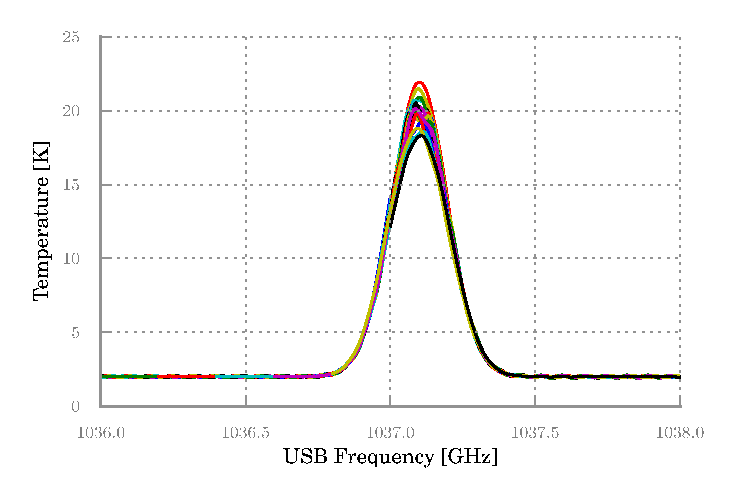
\includegraphics[width=.45\textwidth]{bb-on_narrow}
    }
    \subfigure[\label{fig:calibrated_sbr}
    \footnotesize{Calibration scheme that uses the sideband ratio provided by the model.
    }]{
        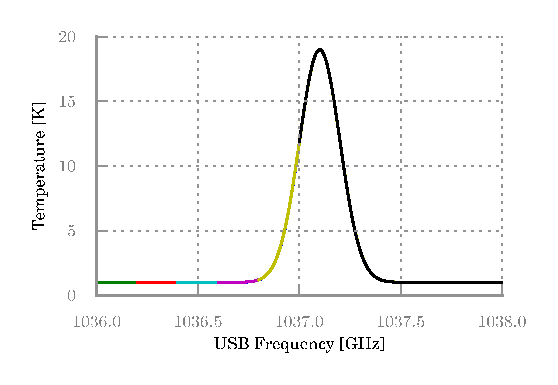
\includegraphics[width=.45\textwidth]{bb-on_corrected-3}
    }
    \caption{\label{fig:calibrated}Simulated spectra.
    Each LO tuning brings its own set of standing waves that modulate the couplings to the different sources.
    Without knowledge of these couplings, the calibration is not perfect.
    The model gives us some information that allows us to properly calibrate out all the standing waves.}
\end{figure}

Our model gives us information that is absent from real data: the sideband ratio.
Standing waves, being frequency-dependent, modulate the lower and upper sidebands differently, resulting in an imbalanced ratio between the two sidebands during the folding by the mixer, see figure~\ref{fig:sbr}
By using the sideband ratio predicted by the model, we are able to properly calibrate our simulated spectrum, as illustrated in figure~\ref{fig:calibrated_sbr}.
\begin{figure}[hbtp]
    \centering
    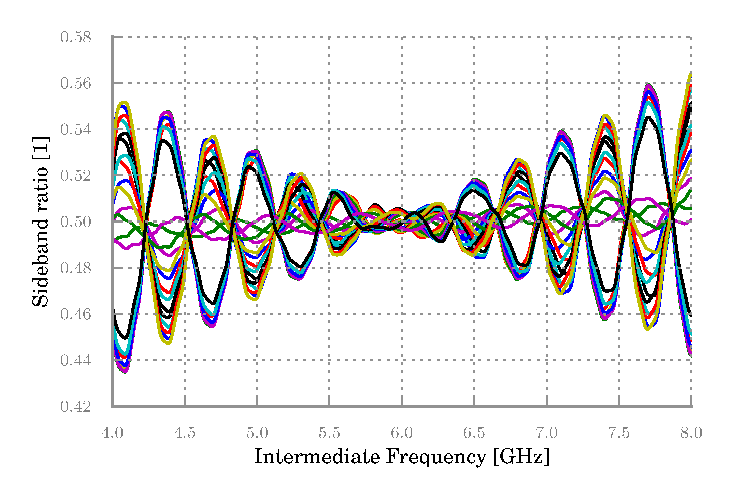
\includegraphics{sbr}
    \caption{\label{fig:sbr}Simulated sideband ratio for a diplexer band of HIFI at 25 different LO~frequencies.
    The sideband ratio is defined in terms of the LSB and USB gains as $G_\text{USB}/(G_\text{LSB} + G_\text{USB})$.  Its ideal value is 0.5; above 0.5, the channel is USB-dominated, and under 0.5 it is LSB-dominated.
    The sideband ratio varies quickly over the IF, as several standing wave patterns beat and modulate each other.
    The \SI{620}{\mega\hertz}-wide periodic modulation comes from the standing wave between the mixers and the closest roof-top mirrors of the diplexer assemblies.  The wide envelop results from the fact that the diplexer tuning is optimal at the center of the IF and degrades on the edges.  We can also see a~\SI{150}{\mega\hertz} pattern that correspond to the LO-mixer cavities.}
\end{figure}





%=============================================================================

\section{Conclusion}
We have designed and implemented a framework to model the interferences, and therefore the standing waves, in any coherent instrument.
The model produces results that are qualitatively consistent with many HIFI observations.
We showed that the model can give us information (notably the sideband ratio) that we can use to better calibrate data.
By modeling more accurately the networks, we are expecting to reproduce quantitatively HIFI data.
This would allow us to significantly reduce the uncertainties in the calibration.

%=============================================================================

\printbibliography
\end{document}
